\section{Lecture 16: FIR Filter Design Using Least-Squares}

\subsection{Ideal Filters}
%
So far, we've discussed generic systems with a transfer function or
frequency response, which transform some input signal into an output
signal. In the time domain, this involves convolution of the input
signal with an impulse response, while in the frequency domain, the
transfer function or frequency response is multiplied by the frequency
domain representation of the input signal, i.e.
%
\begin{displaymath}
  y[n] = x[n] * h[n] \quad\Longleftrightarrow\quad
  Y(\omega) = X(\omega)H(\omega) \,,
\end{displaymath}
%
where the magnitude and phase of the complex $Y(\omega)$ can be written
%
\begin{displaymath}
  |Y(\omega)| = |X(\omega)| \cdot |H(\omega)|
  \quad\mathrm{and}\quad
  \angle Y(\omega) = \angle X(\omega) + \angle H(\omega) \,,
\end{displaymath}
%
respectively. These are the two quantities that are plotted in a Bode
plot. A common frequency response that we've encountered is the
low-pass filter, given by
%
\begin{displaymath}
  H_\mathrm{lp}(\omega) = \rect{\frac{\omega}{\omega_c}} =
  \left\{\begin{array}{ccl}
  1 & & -\omega_c \leq \omega \leq \omega_c \\
  0 & & \mathrm{otherwise}
  \end{array}\right. \,,
\end{displaymath}
%
i.e. only the frequencies in the ``pass'' region are allowed through,
and are completely unmodified (not phase shifted).
We've also see that a pulse in the frequency-domain is a $\sinc$ in
the time domain, such that
%
\begin{displaymath}
  h_\mathrm{lp}[n] = \frac{\sin\left(\omega_c n\right)}{\pi n}
  = \sinc(\omega_c n) \,.
\end{displaymath}
%
Implementing this idealised low-pass filter presents us with some problems.
The first is that the $\sinc$ is not causal, and the second is that it
has infinite duration, neither of which we can realise in a physical system.\\

We have previously seen that for an ideal delay filter,
%
\begin{displaymath}
  h_\mathrm{d}[n] = \delta[n-n_d]
  \quad\Longleftrightarrow
  H_\mathrm{d}(\omega) = \ex{-\im\omega n_d} \,,
\end{displaymath}
%
where $n_d$ is some constant delay. The magnitude and phase of this
frequency response are simply
%
\begin{displaymath}
  |H_\mathrm{d}(\omega)| = 1 \quad\mathrm{and}\quad
  \angle H_\mathrm{d}(\omega) = -\omega n_d
\end{displaymath}
%
since $H(\omega) = |H(\omega)|\ex{\im\angle H(\omega)}$. We see that
the phase shift is a linear function of $\omega$; a filter with linear
phase then effectively delays the output by some number of units. This
isn't distortion since all frequencies are delayed by the same amount,
and the resultant interference pattern doesn't change, i.e. the output
sequence is just the input sequence shifted in time. In many cases, we
can't obtain a filter with zero phase (a filter which doesn't introduce
a delay into the signal). However, we are usually content with linear
phases.\\
%
Modifying our low-pass filter to have linear phase,
%
\begin{displaymath}
  H_\mathrm{lp}(\omega)
  = \ex{-\im\omega n_d}\rect{\frac{\omega}{\omega_c}} =
  \left\{\begin{array}{ccl}
  \ex{-\im\omega n_d} & & -\omega_c \leq \omega \leq \omega_c \\
  0 & & \mathrm{otherwise}
  \end{array}\right.
  \quad\Longleftrightarrow\quad
  h_\mathrm{lp}[n] = \frac{\sin(\omega_c(n-n_d))}{\pi(n-n_d)} \,.
\end{displaymath}
%
This suggests that, for the low-pass filter, we might be able to introduce
some delay $n_d$ which is large enough that the impulse response shifts
over to the right enough that $h[n-n_d]$ for $n<0$ is sufficiently
small as to not yield significant deviations in the output signal from the
desired output signal. However, while we've addressed the impulse response
not being causal, we've done nothing to address the infinite duration of
the impulse response.

\subsection{Group Delay}
%
We define the \textbf{group delay} as
%
\begin{displaymath}
  \tau_g = -\ddx{\omega} \arg H(\omega) \,.
\end{displaymath}
%
Consider the magnitude and phase of the frequency response of a
low-pass filter in panes (a) and (c) of Figure
\ref{fig::lecture_16_amplitude_response}. The discontinuities in the phase 
arise from the non-smooth points in the magnitude, i.e. where the frequency
response changes sign. Neither of these are desirable to work with from
an analytic point of view. Rather, the amplitude and ``properly unwrapped''
phase-shift, $A(\omega)$ and $\phi(\omega)$, respectively, are plotted in
panes (b) and (d) of Figure \ref{fig::lecture_16_amplitude_response},
which are both smooth and continuous,
%
\begin{displaymath}
  A(\omega) = \pm |H(\omega)| \quad\mathrm{and}\quad
  \phi(\omega) = \arg H(\omega) \,.
\end{displaymath}
%
We see then that since $\phi(\omega)$ is linear for an ideal filter, if the
group delay is approximately a constant, then the phase delay of the filter
is approximately linear.
%
\begin{figure}[H]
  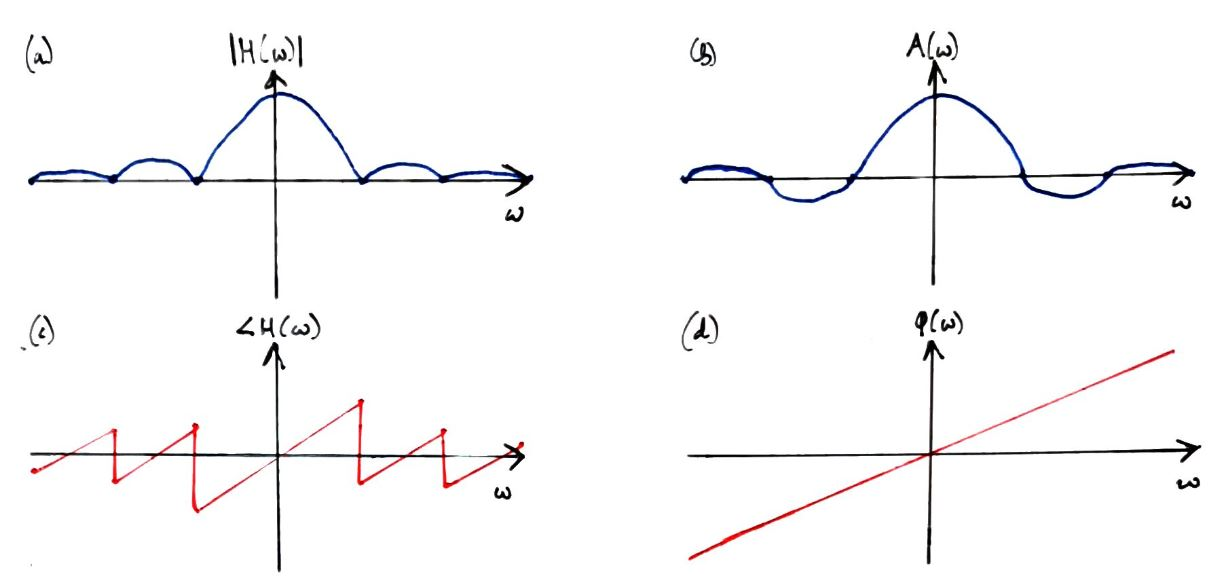
\includegraphics[width=\textwidth]{images/lecture_16_amplitude_response.JPG}
  \caption{In panes (a) and (c), the magnitude and phase responses of a filter,
    $|H(\omega)|$ and $\angle H(\omega)$ respectively, are shown. Note the
    discontinuities in $\angle H(\omega)$ which coincide with the points
    at which the magnitude response is not smooth. Panes (b) and (d) present
    the amplitude response and properly unwrapped phase-shift, $A(\omega)$ and
    $\phi(\omega)$ respectively, for the same filter; note that both are
    smooth and continuous, making their analytic treatment simpler.
  }
  \label{fig::lecture_16_amplitude_response}
\end{figure}

\subsection{Filter Design Process}
%
We have some desired frequency response, $H_\mathrm{des}(\omega)$, and we'd
like to approximate this as closely as possible using an approximate frequency
response which is constrained in form. Our filter design process can then
be enumerated as follows:
%
\begin{enumerate}
\item Choose a desired frequency response, $H_\mathrm{des}(\omega)$.
\item Choose an allowable class of filters (e.g. length-$N$ FIR filter).
\item Choose a measure of quality of the approximate filter.
\item Apply a method or algorithm which returns the optimal parameters of the
  filter.
\item Choose the best realisation of the filter (e.g. optimisation the implementation
  subject to some constraints, such as noise).
\end{enumerate}
%
In this lecture, we'll constrain our discussion to real, causal and digital filters
of the form
%
\begin{displaymath}
  H(z) = \frac{
    b_0 + b_1z^{-1} + b_2z^{-2} + \hdots + b_Mz^{-M}
  }{
    1 + a_1z^{-1} + a_2z^{-2} + \hdots + a_Nz^{-N}
  } \,,
\end{displaymath}
%
that have linear phase. If $\{a_i\} = 0$, then we have a FIR, or
\textbf{finite impulse response} filter, which by definition has no poles, otherwise we
have an IIR, or \textbf{infinite impulse response} filter. In general, we're
interested in the problem
%
\begin{displaymath}
  \min_{\{a\},\{b\}} \fnorm{E(z)} = \fnorm{H_\mathrm{des}(z) -
  \frac{
    b_0 + b_1z^{-1} + b_2z^{-2} + \hdots + b_Mz^{-M}
  }{
    1 + a_1z^{-1} + a_2z^{-2} + \hdots + a_Nz^{-N}
  }
  } \,.
\end{displaymath}
%
Consider $[n]$, a length-$N$ FIR filter, and assume it has linear phase
$\phi(\omega) = k_1 + k_2\omega$. Then,
%
\begin{align*}
  H(\omega) &= \sum_{n=0}^{N-1}h[n]\ex{-\im\omega n}
  = \ex{\im\omega M}\sum_{n=0}^{N-1}h[n]\ex{-\im\omega n}\ex{\im\omega M} \\
  &= \ex{\im\omega M}\sum_{n=0}^{N-1}h[n]\ex{\im\omega(M - n)} \,,
\end{align*}
%
where we've introduced the constant $M = \frac{N-1}{2}$. Now we note that there's
some kind of symmetry about the middle point in $h[n]$, e.g.
%
\begin{displaymath}
  h[0]\ex{\im\omega M} = h[0]\ex{\im\omega\frac{N-1}{2}} \,,
\end{displaymath}
%
and
%
\begin{displaymath}
  h[N-1]\ex{\im\omega M - \frac{N-1}{2}} = h[N-1]\ex{\im\omega\frac{N-1}{2} - \frac{N-1}{2}}
  = h[N-1]\ex{-\im\omega\frac{N-1}{2}} = h[N-1]\ex{-\im\omega M} \,.
\end{displaymath}
%
Now, we can generalise this,
%
\begin{align*}
  H(\omega) &= \ex{\im\omega M}\left(
  h[0]\ex{\im\omega M} + h[1]\ex{\im\omega(M-1)} + \hdots h[N-2]\ex{-\im\omega(M-1)} + h[N-1]\ex{-\im\omega M}
  \right) \\
  &= \ex{\im\omega M}(
  (h[0] + h[N-1])\cos(\omega M) + \im(h[0] - h[N-1])\sin(\omega M)\\
  &+ (h[1] + h[N-2])\cos(\omega (M - 1)) + \im(h[1] - h[N-2])\sin(\omega (M-1))\\
  &+ \hdots) \,.
\end{align*}
%
This slightly messy form is useful since we have a prefactor of $\ex{\im\omega M}$, i.e.
a linear phase, and a sum of sinusoids. We're now interested in when this can
be put in the form
%
\begin{displaymath}
  H(\omega) = A(\omega) \ex{\im(k_1 + k_2\omega)} \,,
\end{displaymath}
%
where $A(\omega)$ is real. Through comparison of terms, we see that the previous
expression for $H(\omega)$ is strictly real when the sine terms are zero, i.e.
when $h[n] = h[N-n-1]$, which implies that the filter must be symmmetric about
its middle element. Then
%
\begin{displaymath}
  A(\omega) = \sum_{m=0}^{M-1}2h[m]\cos(\omega(M-m)) + h[M]
\end{displaymath}
%
if $M$ is odd. So, if we have an odd-length filter which is symmetric about its
middle element, the filter will automatically have linear phase $\ex{-\im\omega M}$.
Similarly, if $M$ is even, there's a slightly different formula for the amplitude,
%
\begin{displaymath}
  A(\omega) = \sum_{m=0}^{\frac{N}{2}-1}2h[m]\cos(\omega(M-m)) \,,
\end{displaymath}
%
i.e. there's no DC term since the middle of the filter now occurs between
two filter values.\\

Now, since we know that choosing a symmetric impulse response we obtain a filter
with linear phase, we need only concern ourselves with their amplitude response.
There are four distinct types of filter with linear phase (i.e. their amplitude
responses are given by a summation of cosines), numbered Types I, II, III, and IV.
These are depicted in Figure \ref{fig::lecture_16_filter_types}.
Note that while Types II and IV appear to
contravene our requirement that the DTFT is $2\pi$-periodic, it's the magnitude
reponse that needs to be $2\pi$-periodic, rather than the amplitude response, which
is clearly satisfied here.\\
%
\begin{figure}[H]
  \includegraphics[width=\textwidth]{images/lecture_16_filter_Types.JPG}
  \caption{The four types of digital filter. In pane (a), a Type I filter
    is shown. Its amplitude response resembles a low-pass filter and is
    generated by a symmetric impulse response with an odd number of taps. In pane (b),
    a Type II filter is shown. Its amplitude response resembles a low-pass filter
    and is generated by a symmetric impulse response with an even number of taps.
    In pane (c), a Type III filter is shown. Its amplitude response resembles
    a band-pass filter and is generated by an antisymmetric impulse response
    with an odd number of taps. Finally, in pane (d) a Type IV filter is
    shown. Its amplitude response resembles a high-pass filter  and is generated
    by an antisymmetric impulse response with an even number of taps.
  }
  \label{fig::lecture_16_filter_types}
\end{figure}

\subsection{Quantifying the Quality of a Filter}
%
Consider some low-pass filter with cutoff frequency $\omega_c$. Typically,
we can't construct a filter with this idealised dropoff from the pass-band
to the stop-band at $\omega_c$. Rather, there's some transition region where
the pass-band transitions to the stop-band in some fashion. We'll refer to
the transition region by the domain $[\omega_1,\omega_2]$. One way we can
construct the filter is to specify its desired behaviour over the transition
region (see pane (b) of Figure \ref{fig::lecture_16_filter_quality}).
Alternatively, we can concern ourselves with the
quality of the pass-band and stop-band, and express no preference in the
form of the filter in the transition region (see pane (c) of
Figure \ref{fig::lecture_16_filter_quality}).\\
%
\begin{figure}[H]
  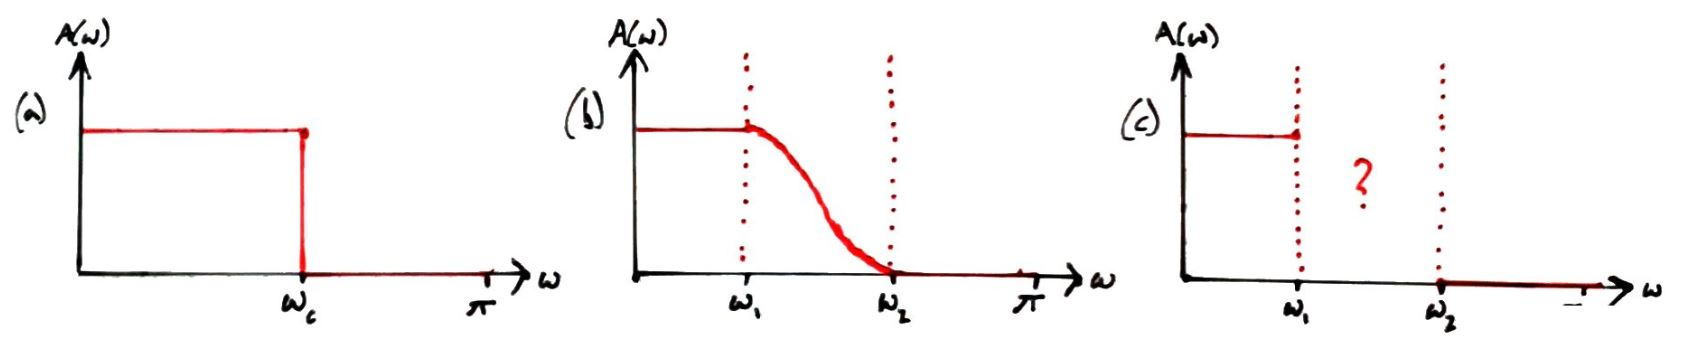
\includegraphics[width=\textwidth]{images/lecture_16_filter_quality.JPG}
  \caption{In pane (a), an idealised low-pass filter is shown with
    exact cutoff frequency of $\omega_c$. In pane (b), the behaviour of
    the transition region has been specified at the expense of poorer
    pass- and stop-band regions. In pane (c), the quality of the
    pass- and stop-band regions is prioritised, at the cost of
    having no control over the filter's form in the transition region.
  }
  \label{fig::lecture_16_filter_quality}
\end{figure}
%
We have a few metrics to quantify the quality of our constructed filter:
%
\begin{itemize}
\item (\textbf{Least-Square Approximation}) Average or squared error in the
  frequency domain. These are simple to implement but the filter may behave
  poorly in the transition region.
\item (\textbf{Chebyshev Approximation}) Maximum error over the pass-band or
  stop-band. These are more controllable in terms of the ripple of the filter,
  although it may take longer for the design process to converge.
\item (\textbf{Butterworth Filters}) A Taylor Series approximation to the
  desired response, sometimes referred to as ``maximally flat'', i.e. the function
  and all of its derivatives are as close to the desired filter as possible
  in a Taylor Series sense.
\end{itemize}

\subsection{Frequency Sampling Design of FIR Filters}
%
We now discuss the means by which we obtain the impulse response of the filter
from its amplitude response. We begin by taking $N$ equally spaced points on
the domain $[0,2\pi]$, i.e. the points $\omega_k = \frac{2\pi k}{N}$, where $N$
is the filter length. These samples are precisely those points that would be
taken with the DFT; the amplitude response can be acquired from the DTFT, which
the DFT samples. So, we can get an FIR filter that exactly interpolates these
samples with the IDFT,
%
\begin{displaymath}
  h[n] = \frac{1}{N}\sum_{k=0}^{N-1}H[k]\ex{\frac{\im 2\pi k n}{N}} \,.
\end{displaymath}
%
For a Type I filter, since we only care about the amplitude response,
%
\begin{displaymath}
  h[n] = \frac{1}{N}\left[
    A[0] + \sum_{k=1}^M 2A[k]\cos\left(\frac{2\pi(n-M)k}{N}\right)
  \right] \,.
\end{displaymath}
%
\begin{exmp}
  Consider a low-pass filter where $N=15$ (i.e. $M = \frac{N-1}{2} = 7$), and we
  have a desired cutoff frequency at $A_\mathrm{des}(\omega) = 0.4\pi$. The
  code given in \texttt{scripts/lecture\_16\_fir.py} constructs an approximation
  to the desired filter through use of frequency sampling. Its output is visualised
  in Figure \ref{fig::lecture_16_fir}.
  %
  \begin{figure}[H]
    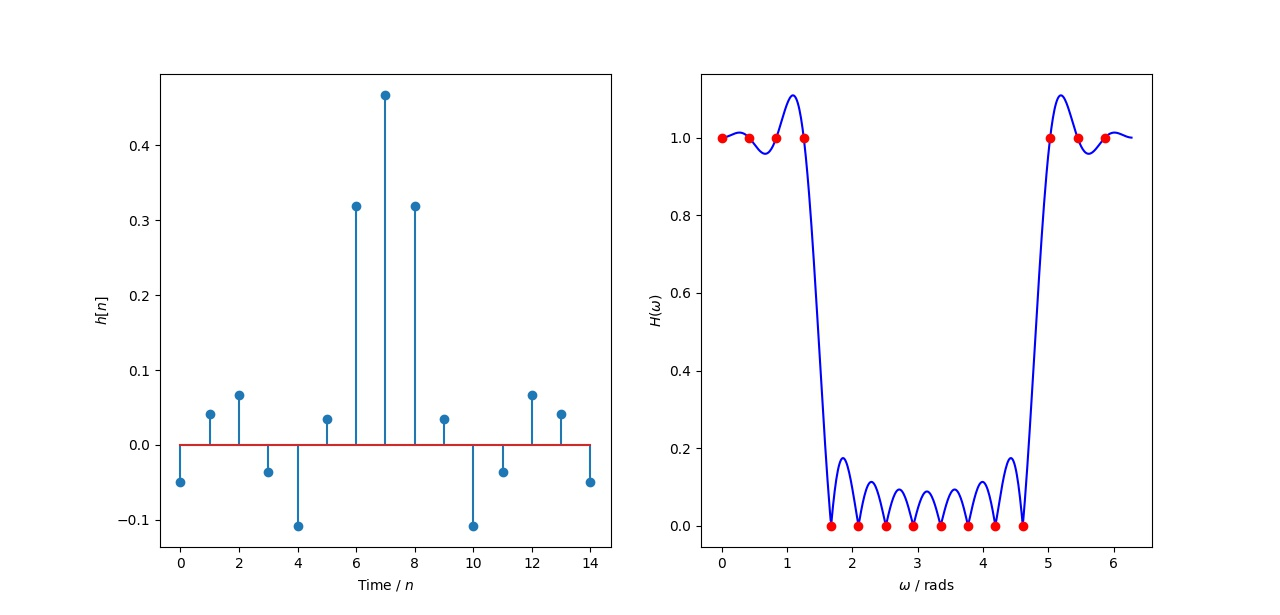
\includegraphics[width=\textwidth]{images/lecture_16_fir.JPG}
    \caption{The impulse response (left) and its frequency response
      (right) of a $15$-tap FIR filter constructed by frequency sampling.
      The sampled points are shown on the right as red circles; note that
      the interpolated frequency response passes exactly through these
      points.
    }
    \label{fig::lecture_16_fir}
  \end{figure}
  %
\end{exmp}
%
Consider the case where we wish to generate an $N$-tap FIR filter, but
using $L>N$ samples of the amplitude response. This yields an overdetermined
system of equations, and consequently has no unique solution. However,
we can use the method of ordinary least squares to find an approximate
solution,
%
\begin{displaymath}
  E = \sum_{k=0}^{L-1}\fnorm{A(\omega_k) - A_\mathrm{des}(\omega_k)}^2 \,,
\end{displaymath}
%
where $\omega_k = 2\pi k/L$. By recalling Parseval's Theorem, it transpires
that this error can be interpreted in the time-domain,
%
\begin{displaymath}
  E = \sum_{k=0}^{L-1} \fnorm{h[n] - h_\mathrm{des}[n]}^2 \,,
\end{displaymath}
%
where $h_\mathrm{des}[n]$ is the length-$L$ FIR filter which goes through
the $L$ samples (as per the previous example). To minimise, we then choose
$h[n]$ to agree with $h_\mathrm{des}[n]$ on the middle $N$ filter taps, i.e.
like truncating $h_\mathrm{des}[n]$. So we find the best length-$L$ filter,
and ``chop out'' the middle $N$ taps, which provides us with the best
length-$N$ approximation to $h_\mathrm{des}[n]$. This filter will have
a different frequency response to one constructed from $N$ samples of
the desired amplitude response, but ultimately will be better since
it provides an improved solution to the least-squares minimisation.

\subsection{Non-Uniform Frequency Sampling Design of FIR Filters}
%
It's possible to use $N$ non-uniformly spaced samples of the
amplitude response to construct the corresponding impulse response, but we
would not be able to use the IDFT for this. It's best to think about
this in terms of matrix algebra, where
%
\begin{displaymath}
  A(\omega) = \sum_{m=0}^{M-1}2h[n]\cos(\omega(M-m)) + h[M]
\end{displaymath}
%
is written
%
\begin{displaymath}
  \left[\begin{array}{c} A(\omega_0) \\ A(\omega_1) \\ \vdots \\ A(\omega_{L-1})\end{array}\right]
  =
  \left[\begin{array}{cccc}
      2\cos(\omega_0 M) & 2\cos(\omega_0 (M-1)) & \hdots & 1 \\
      2\cos(\omega_1 M) & 2\cos(\omega_1 (M-1)) & \hdots & 1 \\
      \vdots & \vdots & \ddots & \vdots \\
      2\cos(\omega_{L-1} M) & 2\cos(\omega_{L-1} (M-1)) & \hdots & 1      
    \end{array}\right]
  \left[\begin{array}{c} h[0] \\ h[1] \\ \vdots \\ h[M]\end{array}\right]
\end{displaymath}
%
\begin{displaymath}
  \mathbf{a} = \mathbf{Fh} \,,
\end{displaymath}
%
where $\mathbf{a}\in\mathbb{R}^L$, $\mathbf{h}\in\mathbb{R}^{M+1}$ and
$\mathbf{F}\in\mathbb{R}^{L\times(M+1)}$. If $\mathbf{F}$ is square, i.e.
$M+1 = L$, then $\mathbf{h} = \mathbf{F}^{-1}\mathbf{a}$, otherwise the
least-squares solution requires that the pseudoinverse be used,
%
\begin{displaymath}
  \mathbf{h} = \left(\mathbf{F}^\top\mathbf{F}\right)^{-1}\mathbf{F}^\top\mathbf{a} \,.
\end{displaymath}
%
Being able to use non-uniform samples of the amplitude response is useful
for directing our sampling of the amplitude response to those regions that
we're particularly concerned about replicating. For instance, if we'd like
the pass-band, which terminates at $\omega_1$, and the stop-band, which
begins at $\omega_2$, to be as close to the desired amplitude response as
possible, we can direct all of our sampling to these regions, at the cost
of placing no constraints on the transition region,
$\omega_1\leq \omega \leq\omega_2$. Similarly, if there are certain
points of the desired amplitude response that we really want to replicate
as closely as possible, we can introduce some weights into the least-squares
minimisation
%
\begin{displaymath}
  E = \sum_{k=0}^{L-1}w_k\fnorm{A(\omega_k) - A_\mathrm{des}(\omega_k)}^2 \,,
\end{displaymath}
%
and in terms of the matrix formulation,
%
\begin{displaymath}
  \mathbf{h} = \left(\mathbf{F}^\top\mathbf{F}\right)^{-1}
  \mathbf{F}^\top\mathbf{W}\mathbf{a} \,.
\end{displaymath}
%
where $\mathbf{W}$ is the diagonal weight matrix.
